\documentclass[12pt]{article}
\usepackage[left=1in, right=1in, top=0.5in, bottom=1.0in]{geometry}
\usepackage{graphicx}
\usepackage[utf8]{inputenc}
\usepackage{wrapfig}
\usepackage{tikz}
\usepackage{amsmath}
\usetikzlibrary{positioning}
\usepackage{geometry}

\usepackage{indentfirst}
\setlength{\parskip}{1em}
\renewcommand{\baselinestretch}{1.5}

\title{Neural Networks\vspace{-3ex}}
\author{Gautom Das, Liam DeVoe, Nate Kelkay}
\date{}

\begin{document}
\maketitle
\vspace{-12ex}
\section*{Introduction}
\vspace{-3ex}
Before we begin, we would like to briefly go over words that are commonly thrown around but \textbf{may not} be used interchangeably in the discussion of neural networks. As we have already discussed artificial intelligence and  machine learning —any algorithm with the ability to learn— we will start by defining deep learning: a subset of machine learning that take advantage of neural networks. The different fields relate to one another as subfields as seen below:

\begin{figure}[h]
	\centering
	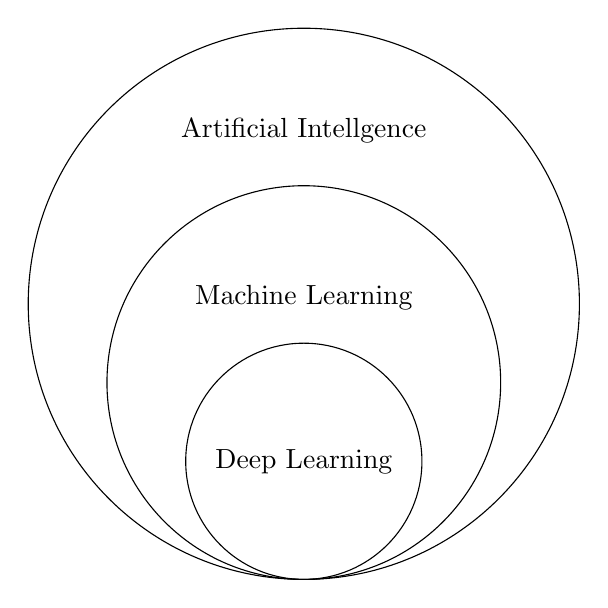
\begin{tikzpicture}
	\draw (0,0) circle (3.5cm);
	
	\draw (0,-1) circle (2.5cm);
	
	\draw (0,-2) circle (1.5cm);
	\node[text width=5cm, align=center] at (0,2.2) 
    {Artificial Intellgence};
    \node[text width=5cm, align=center] at (0,0.08) 
    {Machine Learning};
    \node[text width=5cm, align=center] at (0,-2) 
    {Deep Learning};
    
    
	\end{tikzpicture}
	\caption{Visual of the subfields.}
	\label{fig:vis}
\end{figure}

\section*{Field}
Let's start with a single neuron from the brain. Dendrites feed information into it, then there is the body of the neuron that performs some 'biology' operation on the inputs then outputs this information with its axons.

\begin{figure}[h]
\center
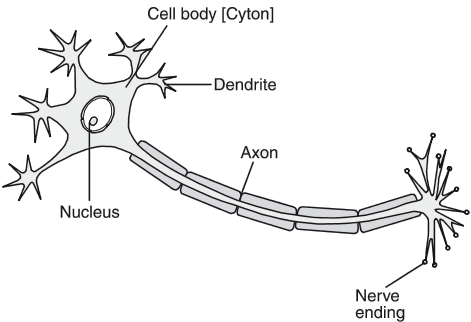
\includegraphics[width=0.65\textwidth]{12img}
	\caption{Diagram of a dendrite}
	\label{fig:vis}
\end{figure}

With this understanding, the following model for a neuron may be developed. 


\begin{center}
	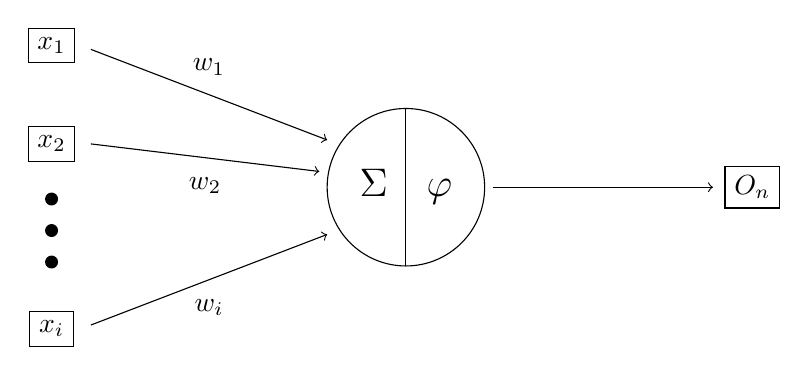
\begin{tikzpicture}
	\draw (0,0) circle (1cm);
	\draw [->] (-4,1.75) -- node[label= above:$w_1$] {} (-1,0.6);
	\node[draw] at (-4.5,1.8) {$x_1$};
	
	\draw [->] (-4, 0.55) -- node[label= below:$w_2$]  {} (-1.1,0.2);
	\node[draw] at (-4.5, 0.55) {$x_2$};
	
	\draw [fill] (-4.5,-0.15) circle [radius=0.075];
	\draw [fill] (-4.5,-0.55) circle [radius=0.075];
	\draw [fill] (-4.5,-0.95) circle [radius=0.075];
	
	\draw (0,1) -- (0,-1);
	
	\draw [->] (-4,-1.75) -- node[label= below:$w_i$]  {} (-1,-0.6);
	\node[draw] at (-4.5,-1.8) {$x_i$};
	
	\draw [->] (1.1,0) -- (3.9,0);
	\node[draw] at (4.4,0) {$O_n$};
	
	\node[text width=3cm, align=center,font=\Large] at (0,0) 
    {\textbf{$\Sigma \:  \:\:  \varphi$}};
    
    
	\end{tikzpicture}
	
\end{center}

Similar to the biological description for a neuron, this model feeds in information denoted $x_n$, multiplies each input by its own weight denoted $w_n$ then feeds into some function that sums all the information. From there an additional function may be performed on the input and then this value is passed onto the next set of neurons. The formal formula for this neuron also takes advantage of a bias:
$$
O_n = \varphi \Big(\sum_{i=1}^{n}{x_iw_i} + b\Big)
$$ 

This function $\varphi$ is the \textbf{activation function}. An activation is any function that takes some real number and maps it to a constrained function. Common examples are the sigmoid function, $\sigma(x)=\frac{1}{1+e^{-x}}$ and the tanh function. Intuitively, the reason an activation function is needed is because the inputs and weights can theoretically become any number. Without an activation function, very large inputs/weights would dominate the network and skew learning.

Combining many of these networks gives you a perceptron as seen below:
\newline
\newline
\newline
\newline

\tikzset{%
  every neuron/.style={
    circle,
    draw,
    minimum size=1cm
  },
  neuron missing/.style={
    draw=none, 
    scale=4,
    text height=0.333cm,
    execute at begin node=\color{black}$\vdots$
  },
}
\begin{center}
\hspace*{-4.5cm}
\vspace*{.5cm}
\begin{tikzpicture}[x=1.6cm, y=1.5cm, >=stealth, transform canvas={scale=0.75}]

\foreach \m/\l [count=\y] in {1,2,missing,3}
  \node [every neuron/.try, neuron \m/.try] (input-\m) at (0,2.5-\y) {};

\foreach \m [count=\y] in {1, 2,missing,3}
  \node [every neuron/.try, neuron \m/.try ] (hidden-\m) at (2,3.2-\y*1.25) {};

\foreach \m [count=\y] in {1,missing,2}
  \node [every neuron/.try, neuron \m/.try ] (output-\m) at (4,2.0-\y) {};

\foreach \l [count=\i] in {1,2,n}
  \draw [<-] (input-\i) -- ++(-1,0)
    node [above, midway] {$I_\l$};

\foreach \l [count=\i] in {1,2,n}
  \node [above] at (hidden-\i.north) {$H_\l$};

\foreach \l [count=\i] in {1,n}
  \draw [->] (output-\i) -- ++(1,0)
    node [above, midway] {$O_\l$};

\foreach \i in {1,...,3}
  \foreach \j in {1,...,3}
    \draw [->] (input-\i) -- (hidden-\j);

\foreach \i in {1,...,3}
  \foreach \j in {1,...,2}
    \draw [->] (hidden-\i) -- (output-\j);

\foreach \l [count=\x from 0] in {Input, Hidden, Ouput}
  \node [align=center, above] at (\x*2,2.7) {\l \\ layer};

\end{tikzpicture}

\end{center}

\vspace{1ex}

\subsection*{Forward Propagation}
\vspace{-3ex}
A perceptron is our neural network. Inputting the values at the start of the input layer and then running it through the network will give you the predicted output. We can describe the weights of a general vector at any given hidden layer $H_n$:
$$
H_n = w_1i_1 + w_2i_2 + ... + w_ni_n
$$

\vspace{-2ex}
\vspace{-3ex}
\subsection*{Cost Function}
\vspace{-3ex}
Now we have two vectors: the output layer of the model and the expected value. In order to train our model we need to start by evaluating our error. The method that is most commonly used in regression functions is Mean-Squared Error (MSE):
$$
MSE=\frac{1}{n}\sum_{i=1}^{n}(\hat{y}_i-\hat{y})^2
$$
\vspace{0ex}
For different applications there are specific functions that perform better than others. The cost function itself is the average of all the different costs in a training data set. 

\subsection*{Backward Propagation}
Now that we can evaluate our error, we can change our neural network with backpropogation. Let's take a simple example of a network with two neurons:

 \begin{center}
	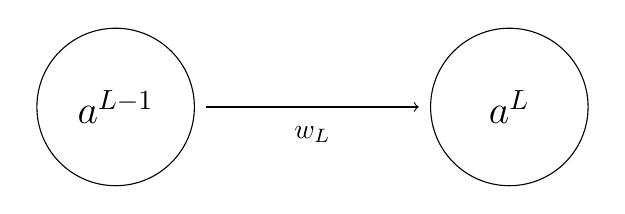
\begin{tikzpicture}
	\draw (-2.5,0) circle (1cm);
	
	\draw (2.5,0) circle (1cm);
	
	
	\draw [->] (-1.35,0) -- node[label= below:$w_L$]  {} (1.35,0);
	
	\node[text width=2cm, align=center,font=\Large] at (-2.5,0) 
    {$a^{L-1}$};
    \node[text width=2cm, align=center,font=\Large] at (2.5,0) 
    {$a^{L}$};
    
	\end{tikzpicture}
	
\end{center}
 
 Let's start by calculation the cost of our last node $a^L$ versus the real output $y$:
 $$
 C = (a^L-y)^2
 $$
 
 From here, we want to figure out how sensitive the cost function is to the weight $w^L$. In more formal terms we want $\frac{\partial C}{\partial w^L}$. Knowing how each value in a neural network is connected we want to first define a relationship between $a^{L-1}$ and $a^L$:
 $$
 z^{L} = w^{L}a^{L-1}+b^{L-1}
 $$
 $$
 a^{L} = \varphi (x^L)
 $$
 
 Now we can establish a clear relationship between the cost and the weight:
 $$
 \frac{\partial C}{\partial w_L} = \frac{\partial z^L}{\partial w_L} \frac{\partial a^L}{\partial z^L} \frac{\partial C}{\partial a^L}
 $$
 
 Doing the specific partial derivatives we can solve each value in our chain rule to get our final value:
 $$\frac{\partial z^L}{\partial w_i} = a^{L-1}$$
 $$\frac{\partial a^L}{\partial z^L} = \varphi'(z^L)$$
 $$ \frac{\partial C}{\partial a^L} = 2(a^L-y)$$
 
 We have now our final cost formula of:
 $$
  \frac{\partial C}{\partial w^L} = a^{L-1} \varphi'(z^L) 2(a^L-y)
 $$
 \newpage
 Our gradient for the function is the average of all of these cost functions in relation to every output and weight/bias:

 
 \[
 \nabla C = \begin{bmatrix} 
      \frac{\partial C}{\partial w^1} \\
      \frac{\partial C}{\partial b^1} \\
    \vdots  \\
     \frac{\partial C}{\partial w^L} \\
      \frac{\partial C}{\partial b^L} \\
    \end{bmatrix}
\]
 
 Finally, we have the gradient descent algorithm. Gradient descent is an iterative algorithm which takes steps to reduce a function. Thus we first have to define a learning rate we call $\alpha$. We also need our cost for the current input. From there given a certain point $\Theta_j$ we can define the best path to reduce its weight as:
 $$
 \Theta_j = \Theta_j - \alpha\frac{\partial }{\partial \Theta_j} *C
 $$
 
 This is our gradient descent algorithm. Formally you would combine this with the cost function, but these are the basic building blocks behind neural networks.

\vspace{-4ex}
\section*{Convolutional Neural Networks}
\vspace{-3ex}

For convolutional neural networks, the goal of the 'convolutions' is to convert the images to an array of features. These networks consists of two steps: creating a feature map and pooling the network. The feature map is created by multiplying some matrix over a given image. Different matrixes are designed to highlighted different feature types. From there, pooling consists of taking the max number in a matrix of pixels. This reduces the image size. From there the final images are 'flattened' by converting it to a 1D array and finally fed into a generic neural network.


\vspace{-4ex}
\section*{Frameworks}
\vspace{-3ex}

There are two different neural network frameworks that stand king but both have their strengths and weaknesses: TensorFlow/Keras and PyTorch. TensorFlow was built on the idea that you build a graph of the neural network at run time and then use this neural network when the computation is finished. PyTorch on the other hand uses something known as dynamic graphs. During the run-time of the program, PyTorch actively defines its graph as its being run. This allows for the neural network to actually change shape is desired by the researcher.

\vspace{-4ex}
\section*{Conclusion}
\vspace{-3ex}
Neural networks are a very impressive form of artificial intelligence but can only be used for specific tasks. It is not a general form of AI.

%%%%%%%%%%%%%%%%%%%%%%%%%%
%%%%%%%%%%%%%%%%%%%%%%%%%%
%%%%%%%%%%%%%%%%%%%%%%%%%%
%%%%%%%%%%%%%%%%%%%%%%%%%%
%%%%%%%%%%%%%%%%%%%%%%%%%%

\newpage
\nocite*

%%\bibliographystyle{plain}
%% \bibliography{xampl}
\newcommand{\noopsort}[1]{} \newcommand{\printfirst}[2]{#1}
  \newcommand{\singleletter}[1]{#1} \newcommand{\switchargs}[2]{#2#1}
\begin{thebibliography}{10}

\bibitem{article-crossref}
Alex Krizhevsky, Ilya Sutskever, Geoffrey E. Hinton,
\newblock ImageNet Classification with Deep Convolutional
Neural Networks
\newblock {\em \mbox{University of Toronto}}, 2012.

\bibitem{article-full}
Ian Goodfellow, Yoshua Bengio, Aaron C. Courville,
\newblock Deep Learning
\newblock {\em \mbox{MIT Press}}, 2015.


\bibitem{article-minimal}
Peter Norvig, Stuart J. Russell,
\newblock Artificial Intelligence: A Modern Approach
\newblock {\em \mbox{Prentice Hall}}, 1994.

\bibitem{article-crossref}
Trevor Hastie, Robert Tibshirani, Jerome H. Friedman,
\newblock The Elements of Statistical Learning.
\newblock {\em \mbox{Prentice Hall}}, 2001.


\end{thebibliography}

\end{document}
